\documentclass[12pt,letterpaper]{exam}
\usepackage[lmargin=1in,rmargin=1in,tmargin=1in,bmargin=1in]{geometry}
\usepackage{../style/exams}

% -------------------
% Course & Exam Information
% -------------------
\newcommand{\course}{MAT 101: Exam 1}
\newcommand{\term}{Fall -- 2023}
\newcommand{\examdate}{10/11/2023}
\newcommand{\timelimit}{85 Minutes}

\setbool{hideans}{false} % Student: True; Instructor: False

% Fraction Long Division
\usepackage{longdivision}

% -------------------
% Content
% -------------------
\begin{document}

\examtitle
\instructions{Write your name on the appropriate line on the exam cover sheet. This exam contains \numpages\ pages (including this cover page) and \numquestions\ questions. Check that you have every page of the exam. Answer the questions in the spaces provided on the question sheets. Be sure to answer every part of each question and show all your work. If you run out of room for an answer, continue on the back of the page --- being sure to indicate the problem number.} 
%\scores
{
\renewcommand{\arraystretch}{2.5}
\begin{table}[H]
\centering
\begin{tabular}{|cccccc|}
\hline
\multicolumn{1}{|c|}{Question} & \multicolumn{1}{c|}{Points} & \multicolumn{1}{c|}{Score} & \multicolumn{1}{c|}{Question} & \multicolumn{1}{c|}{Points} & Score \\ \hline
\multicolumn{1}{|c|}{1} & \multicolumn{1}{c|}{5} & \multicolumn{1}{c|}{} & \multicolumn{1}{c|}{11} & \multicolumn{1}{c|}{5} &  \\ \hline
\multicolumn{1}{|c|}{2} & \multicolumn{1}{c|}{5} & \multicolumn{1}{c|}{} & \multicolumn{1}{c|}{12} & \multicolumn{1}{c|}{5} &  \\ \hline
\multicolumn{1}{|c|}{3} & \multicolumn{1}{c|}{5} & \multicolumn{1}{c|}{} & \multicolumn{1}{c|}{13} & \multicolumn{1}{c|}{5} &  \\ \hline
\multicolumn{1}{|c|}{4} & \multicolumn{1}{c|}{5} & \multicolumn{1}{c|}{} & \multicolumn{1}{c|}{14} & \multicolumn{1}{c|}{5} &  \\ \hline
\multicolumn{1}{|c|}{5} & \multicolumn{1}{c|}{5} & \multicolumn{1}{c|}{} & \multicolumn{1}{c|}{15} & \multicolumn{1}{c|}{5} &  \\ \hline
\multicolumn{1}{|c|}{6} & \multicolumn{1}{c|}{5} & \multicolumn{1}{c|}{} & \multicolumn{1}{c|}{16} & \multicolumn{1}{c|}{5} &  \\ \hline
\multicolumn{1}{|c|}{7} & \multicolumn{1}{c|}{5} & \multicolumn{1}{c|}{} & \multicolumn{1}{c|}{17} & \multicolumn{1}{c|}{5} &  \\ \hline
\multicolumn{1}{|c|}{8} & \multicolumn{1}{c|}{5} & \multicolumn{1}{c|}{} & \multicolumn{1}{c|}{18} & \multicolumn{1}{c|}{5} &  \\ \hline
\multicolumn{1}{|c|}{9} & \multicolumn{1}{c|}{5} & \multicolumn{1}{c|}{} & \multicolumn{1}{c|}{19} & \multicolumn{1}{c|}{5} &  \\ \hline
\multicolumn{1}{|c|}{10} & \multicolumn{1}{c|}{5} & \multicolumn{1}{c|}{} & \multicolumn{1}{c|}{20} & \multicolumn{1}{c|}{5} &  \\ \hline
\multicolumn{2}{|r}{Points:} & \multicolumn{1}{l}{} & \multicolumn{1}{r}{/100} & \multicolumn{2}{l|}{} \\ \hline
\end{tabular}
\end{table}
}
%\bottomline
\newpage

% ---------
% Questions
% ---------
\begin{questions}

% Question 1
\newpage
\question[5] Find the prime factorizations of the following:
	\begin{enumerate}[(a)]
	\item 396
	\item 440
	\end{enumerate} \pspace

\sol
\begin{enumerate}[(a)]
\item $396= 2 \cdot 2 \cdot 3 \cdot 3 \cdot 11= 2^2 \cdot 3^2 \cdot 11$ \pspace
	\[
	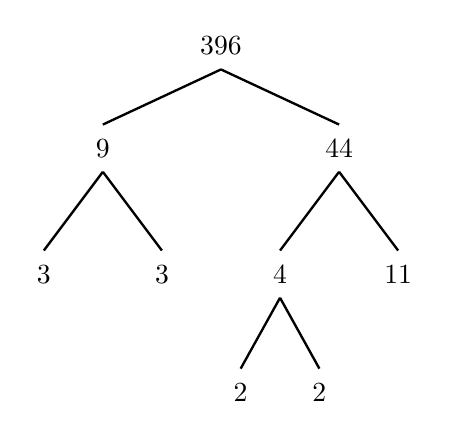
\begin{tikzpicture}
	\node at (0,0) {$396$};
	\node at (-1.5,-1.3) {$9$}; \draw[line width=0.03cm] (-1.5,-1) -- (0,-0.3);
	\node at (1.5,-1.3) {$44$}; \draw[line width=0.03cm] (1.5,-1) -- (0,-0.3);
	
	\node at (-2.25,-2.9) {$3$}; \draw[line width=0.03cm] (-2.25,-2.6) -- (-1.5,-1.6);
	\node at (-0.75,-2.9) {$3$}; \draw[line width=0.03cm] (-0.75,-2.6) -- (-1.5,-1.6);
	\node at (0.75,-2.9) {$4$}; \draw[line width=0.03cm] (0.75,-2.6) -- (1.5,-1.6);
	\node at (2.25,-2.9) {$11$}; \draw[line width=0.03cm] (2.25,-2.6) -- (1.5,-1.6);
	
	\node at (0.25,-4.4) {$2$}; \draw[line width=0.03cm] (0.25,-4.1) -- (0.75,-3.2);
	\node at (1.25,-4.4) {$2$}; \draw[line width=0.03cm] (1.25,-4.1) -- (0.75,-3.2);
	\end{tikzpicture}
	\] \pspace

\item $440= 2 \cdot 2 \cdot 2 \cdot 5 \cdot 11= 2^3 \cdot 5 \cdot 11$ \pspace
	\[
	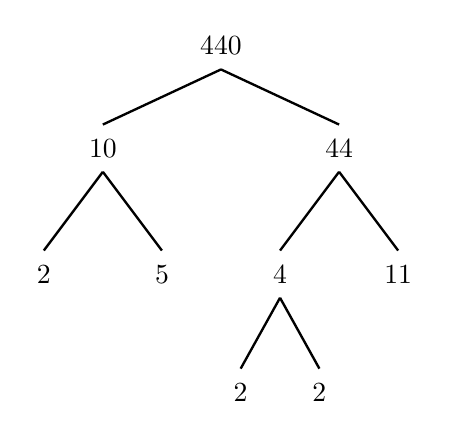
\begin{tikzpicture}
	\node at (0,0) {$440$};
	\node at (-1.5,-1.3) {$10$}; \draw[line width=0.03cm] (-1.5,-1) -- (0,-0.3);
	\node at (1.5,-1.3) {$44$}; \draw[line width=0.03cm] (1.5,-1) -- (0,-0.3);
	
	\node at (-2.25,-2.9) {$2$}; \draw[line width=0.03cm] (-2.25,-2.6) -- (-1.5,-1.6);
	\node at (-0.75,-2.9) {$5$}; \draw[line width=0.03cm] (-0.75,-2.6) -- (-1.5,-1.6);
	\node at (0.75,-2.9) {$4$}; \draw[line width=0.03cm] (0.75,-2.6) -- (1.5,-1.6);
	\node at (2.25,-2.9) {$11$}; \draw[line width=0.03cm] (2.25,-2.6) -- (1.5,-1.6);
	
	\node at (0.25,-4.4) {$2$}; \draw[line width=0.03cm] (0.25,-4.1) -- (0.75,-3.2);
	\node at (1.25,-4.4) {$2$}; \draw[line width=0.03cm] (1.25,-4.1) -- (0.75,-3.2);
	\end{tikzpicture}
	\] 
\end{enumerate}



% Question 2
\newpage
\question[5] Showing all your work, compute the following:
	\begin{enumerate}[(a)]
	\item $\gcd(36, 54)$
	\item $\lcm(36, 54)$
	\end{enumerate} \pspace

\sol 
\begin{enumerate}[(a)]
\item $\gcd(36, 54)= \gcd(2^2 \cdot 3^2, 2 \cdot 3^3)= 2^1 \cdot 3^2= 18$ \pspace
\item $\lcm(36, 54)= \lcm(2^2 \cdot 3^2, 2 \cdot 3^3)= 2^2 \cdot 3^3= 108$
\end{enumerate}



% Question 3
\newpage
\question[5] Showing all your work, compute the following:
	\begin{enumerate}[(a)]
	\item $\gcd \big(2^{40} \cdot 3^{90} \cdot 5^{30} \cdot 17^5,\; 2^{50} \cdot 3^{80} \cdot 11^{20} \cdot 17^5 \big)$ \par\vspace{0.3cm}
	\item $\lcm \big(2^{40} \cdot 3^{90} \cdot 5^{30} \cdot 17^5,\; 2^{50} \cdot 3^{80} \cdot 11^{20} \cdot 17^5 \big)$
	\end{enumerate} \pspace

\sol 
\begin{enumerate}[(a)]
\item $\gcd \big(2^{40} \cdot 3^{90} \cdot 5^{30} \cdot 17^5,\; 2^{50} \cdot 3^{80} \cdot 11^{20} \cdot 17^5 \big)= 2^{40} \cdot 3^{80} \cdot 5^0 \cdot 11^0 \cdot 17^5$ \pspace
	{\footnotesize
	\[
	2^{40} \cdot 3^{80} \cdot 5^0 \cdot 11^0 \cdot 17^5= 230\,751\,647\,806\,918\,333\,113\,422\,816\,410\,774\,688\,737\,564\,386\,243\,989\,471\,232
	\]} \pspace

\item $\lcm \big(2^{40} \cdot 3^{90} \cdot 5^{30} \cdot 17^5,\; 2^{50} \cdot 3^{80} \cdot 11^{20} \cdot 17^5 \big)= 2^{50} \cdot 3^{90} \cdot 5^{30} \cdot 11^{20} \cdot 17^5$
	{\tiny
	\[
	\hspace{-1.5cm} 2^{50} \cdot 3^{90} \cdot 5^{30} \cdot 11^{20} \cdot 17^5= 8\,742\,006\,963\,728\,917\,196\,307\,854\,228\,116\,466\,398\,107\,923\,957\,214\,655\,628\,007\,881\,328\,399\,108\,538\,368\,000\,000\,000\,000\,000\,000\,000\,000\,000\,000
	\]} \pspace
\end{enumerate}



% Question 4
\newpage
\question[5] Showing all your work and simplifying as much as possible, compute the following:
	\begin{enumerate}[(a)]
	\item $\dfrac{99}{140} - \dfrac{29}{42}$ \par\vspace{0.3cm}
	\item $\dfrac{7}{15} - \dfrac{6}{10} + \dfrac{5}{6}$
	\end{enumerate} \pspace

\sol 
\begin{enumerate}[(a)]
\item 
	\[
	\begin{aligned}
	\dfrac{99}{140} - \dfrac{29}{42}&= \dfrac{99}{140} \cdot \dfrac{3}{3} - \dfrac{29}{42} \cdot \dfrac{10}{10} \\[0.3cm]
	&= \dfrac{297}{420} - \dfrac{290}{420} \\[0.3cm]
	&= \dfrac{297 - 290}{420} \\[0.3cm]
	&= \dfrac{7}{420} \\[0.3cm]
	&= \dfrac{7}{420} \cdot \dfrac{1/7}{1/7} \\[0.3cm]
	&= \dfrac{1}{60}
	\end{aligned}
	\] \vfill

\item 
	\[
	\begin{aligned}
	\dfrac{7}{15} - \dfrac{6}{10} + \dfrac{5}{6}&= \dfrac{7}{15} \cdot \dfrac{2}{2} - \dfrac{6}{10} \cdot \dfrac{3}{3} + \dfrac{5}{6} \cdot \dfrac{5}{5} \\[0.3cm]
	&= \dfrac{14}{30} - \dfrac{18}{30} + \dfrac{25}{30} \\[0.3cm]
	&= \dfrac{14 - 18 + 25}{30} \\[0.3cm]
	&= \dfrac{21}{30} \\[0.3cm]
	&= \dfrac{21}{30} \cdot \dfrac{1/3}{1/3} \\[0.3cm]
	&= \dfrac{7}{10}
	\end{aligned}
	\]
\end{enumerate}



% Question 5
\newpage
\question[5] Showing all your work and simplifying as much as possible, compute the following:
	\begin{enumerate}[(a)]
	\item $\dfrac{20}{66} \cdot \dfrac{117}{15}$ \par\vspace{0.3cm}
	\item $\dfrac{\;\;\dfrac{33}{12}\;\;}{\;\;\dfrac{45}{26}\;\;}$
	\end{enumerate} \pspace

\sol 
\begin{enumerate}[(a)]
\item 
	\[
	\dfrac{20}{66} \cdot \dfrac{117}{15}= \dfrac{\cancel{20}^{\,4}}{\cancel{66}^{\,22}} \cdot \dfrac{\cancel{117}^{\,39}}{\cancel{15}^{\,3}}= \dfrac{\cancel{4}^{\,2}}{\cancel{22}^{\,11}} \cdot \dfrac{\cancel{39}^{\,13}}{\cancel{3}^{\,1}}= \dfrac{2}{11} \cdot \dfrac{13}{1}= \dfrac{26}{11}
	\] \pspace

\item 
	\[
	\dfrac{\;\;\dfrac{33}{12}\;\;}{\;\;\dfrac{45}{26}\;\;}= \dfrac{33}{12} \cdot \dfrac{26}{45}= \dfrac{\cancel{33}^{\,11}}{\cancel{12}^{\,6}} \cdot \dfrac{\cancel{26}^{\,13}}{\cancel{45}^{\,15}}= \dfrac{11}{6} \cdot \dfrac{13}{15}= \dfrac{143}{90}
	\]
\end{enumerate}



% Question 6
\newpage
\question[5] Showing all your work and simplifying as much as possible, convert the given improper fractions to a proper fraction and the given proper fraction to an improper fraction:
	\begin{enumerate}[(a)]
	\item $-\frac{129}{7}$
	\item $-11 \frac{7}{10}$
	\end{enumerate} \pspace

\sol 
\begin{enumerate}[(a)]
\item $-\frac{129}{7}= -18 \frac{3}{7}$
	\[
	\intlongdivision{129}{7} % Compare to \longdivision
	\] \pspace

\item $-11 \frac{7}{10}= -\frac{117}{10}$ \pspace
	\[
	-11 \frac{7}{10}= -\left( 11 \frac{7}{10} \right)= - \left( \dfrac{10 \cdot 11 + 7}{10} \right)= -\dfrac{110 + 7}{10}= -\dfrac{117}{10}
	\]
\end{enumerate}



% Question 7
\newpage
\question[5] Showing all your work, simplify the following as much as possible: 
	\[
	\dfrac{x^{-5} y^6}{x^3 y^{-2} (x^3 y^5)^{-2}} \left( \dfrac{xy \big( (x^3 y^{-5})^2 \big)^{-4}}{x^0 y^8 (x^{-5} y^6)^{-12}} \right)^0
	\] \pspace

\sol 
	\[
	\begin{gathered}
	\dfrac{x^{-5} y^6}{x^3 y^{-2} (x^3 y^5)^{-2}} \left( \dfrac{xy \big( (x^3 y^{-5})^2 \big)^{-4}}{x^0 y^8 (x^{-5} y^6)^{-12}} \right)^0 \\[0.3cm]
	\dfrac{x^{-5} y^6}{x^3 y^{-2} (x^3 y^5)^{-2}} \cdot 1 \\[0.3cm]
	\dfrac{x^{-5} y^6}{x^3 y^{-2} (x^3 y^5)^{-2}} \\[0.3cm]
	\dfrac{x^{-5} y^6}{x^3 y^{-2} \cdot x^{-6} y^{-10}} \\[0.3cm]
	\dfrac{x^{-5} y^6}{x^{-3} y^{-12}} \\[0.3cm]
	\dfrac{x^3 y^6 y^{12}}{x^5} \\[0.3cm]
	\dfrac{x^3 y^{18}}{x^5} \\[0.3cm]
	\dfrac{y^{18}}{x^2}
	\end{gathered}
	\]



% Question 8
\newpage
\question[5] Showing all your work, simplify the following as much as possible: 
	\[
	\sqrt{ \dfrac{9 (a^6 b^5)^{1/3}}{a^{-2} b} }
	\] \pspace

\sol 
	\[
	\begin{gathered}
	\sqrt{ \dfrac{9 (a^6 b^5)^{1/3}}{a^{-2} b} } \\[0.3cm]
	\sqrt{ \dfrac{9 a^{6/3} b^{5/3}}{a^{-2} b} } \\[0.3cm]
	\sqrt{ \dfrac{9 a^2 b^{5/3}}{a^{-2} b} } \\[0.3cm]
	\sqrt{ \dfrac{9 a^2 a^2 b^{5/3}}{b} } \\[0.3cm]
	\sqrt{ \dfrac{9 a^4 b^{5/3}}{b} } \\[0.3cm]
	\sqrt{9 a^4 b^{5/3-1} } \\[0.3cm]
	\sqrt{9 a^4 b^{5/3-3/3} } \\[0.3cm]
	\sqrt{9 a^4 b^{2/3} } \\[0.3cm]
	\left( 9 a^4 b^{2/3} \right)^{1/2} \\[0.3cm]
	9^{1/2} a^{4/2} b^{2/3 \cdot 1/2} \\[0.3cm]
	3 a^2 b^{1/3} \\[0.3cm]
	3 a^2 \sqrt[3]{b}
	\end{gathered}
	\]



% Question 9
\newpage
\question[5] Showing all your work, simplify the following as much as possible:
	\begin{enumerate}[(a)]
	\item $\sqrt{24}$
	\item $\sqrt[3]{24}$
	\end{enumerate} \pspace

\sol 
\begin{enumerate}[(a)]
\item $\sqrt{24}= \sqrt{4 \cdot 6}= 2 \sqrt{6}$ \quad {\itshape or} \quad $\sqrt{24}= \sqrt{2^3 \cdot 3}= 2 \sqrt{2^1 \cdot 3}= 2 \sqrt{6}$ \pspace

\item $\sqrt[3]{8 \cdot 3}= 2 \sqrt[3]{3}$ \quad {\itshape or} \quad $\sqrt[3]{24}= \sqrt[3]{2^3 \cdot 3}= 2^1 \sqrt[3]{3}= 2 \sqrt[3]{3}$
\end{enumerate}



% Question 10
\newpage
\question[5] Showing all your work and simplifying as much as possible, convert the following decimal number $0.\overline{23}$ to a fraction. \pspace

\sol Suppose that $N= 0.\overline{23}= 0.2323232323232323\overline{23}$. We have\dots
	\begin{table}[!ht]
	\centering\small
	\begin{tabular}{rccc}
	& $100N$ & $=$ & $23.2323232323232323\overline{23}$ \\ 
	$-$ & $N$ & $=$ & $\phantom{2}0.2323232323232323\overline{23}$ \\ \hline
	& $99N$ & $=$ & $23$ \\[0.1cm]
	& $N$ & $=$ & $\frac{23}{99}$
	\end{tabular}
	\end{table} \par

	\[
	0.\overline{23}= \dfrac{23}{99}
	\] 



% Question 11
\newpage
\question[5] Showing all your work and simplifying as much as possible, compute the following:
	\begin{enumerate}[(a)]
	\item $(8 - 6i) - (5 - 9i)$
	\item $\dfrac{1 - 4i}{-4 + 5i}$
	\end{enumerate} \pspace

\sol 
\begin{enumerate}[(a)]
\item 
	\[
	(8 - 6i) - (5 - 9i)= 8 - 6i - 5 + 9i= (8 - 5) + (-6i + 9i)= 3 + 3i
	\] \pspace

\item 
	\[
	\begin{gathered}
	\dfrac{1 - 4i}{-4 + 5i}= \dfrac{1 - 4i}{-4 + 5i} \cdot \dfrac{-4 - 5i}{-4 - 5i} \\[0.3cm]
	\dfrac{(1 - 4i)(-4 - 5i)}{(-4 + 5i)(-4 - 5i)} \\[0.3cm]
	\dfrac{-4 - 5i + 16i + 20i^2}{16 + 20i - 20i - 25i^2} \\[0.3cm]
	\dfrac{-4 - 5i + 16i + 20(-1)}{16 + 20i - 20i - 25(-1)} \\[0.3cm]
	\dfrac{(-4 - 20) + (-5i + 16i)}{(16 + 25) + (20i - 20i)} \\[0.3cm]
	\dfrac{-24 + 11i}{41} \\[0.3cm]
	-\frac{24}{41} + \frac{11}{41}\,i
	\end{gathered}
	\]
\end{enumerate}



% Question 12
\newpage
\question[5] Showing all your work, compute the following:
	\begin{enumerate}[(a)]
	\item 67\% of 7690
	\item 0.1\% of 4500
	\end{enumerate} \pspace

\sol 
\begin{enumerate}[(a)]
\item 
	\[
	\text{67\% of 7690}= 7690 (0.67)= 5152.3
	\] \pspace

\item 
	\[
	\text{0.1\% of 4500}= 4500 (0.001)= 4.5
	\]
\end{enumerate}



% Question 13
\newpage
\question[5] Showing all your work, compute the following:
	\begin{enumerate}[(a)]
	\item 95 increased by 108\%
	\item 720 decreased by 35\%
	\end{enumerate} \pspace

\sol 
\begin{enumerate}[(a)]
\item 
	\[
	\text{95 increased by 108\%}= 95 (1 + 1.08)= 95(2.08)=  197.6
	\] \pspace

\item 
	\[
	\text{720 decreased by 35\%}= 720(1 - 0.35)= 720(0.65)= 468
	\]
\end{enumerate}



% Question 14
\newpage
\question[5] Given the following course grade components, weights, and student scores, compute the student's course average. 
	\begin{table}[H]
	\centering
	\begin{tabular}{lcc}
	Grade Component & Component Value & Student Grade \\ \hline
	Participation & 5\% & 85\% \\
	Homework & 40\% & 81\% \\
	Project & 15\% & 74\% \\
	Midterm & 15\% & 92\% \\
	Final & 25\% & 86\%
	\end{tabular}
	\end{table} \pspace

\sol 
	\[
	\begin{aligned}
	\text{Course Average}&= \dfrac{\sum \text{weight} \cdot \text{value}}{\sum \text{weights}} \\[0.3cm]
	&= \dfrac{0.05 \cdot 0.85 + 0.40 \cdot 0.81 + 0.15 \cdot 0.74 + 0.15 \cdot 0.92 + 0.25 \cdot 0.86}{0.05 + 0.40 + 0.15 + 0.15 + 0.25} \\[0.3cm]
	&= \dfrac{0.0425 + 0.324 + 0.111 + 0.138 + 0.215}{1} \\[0.3cm]
	&= \dfrac{0.8305}{1} \\[0.3cm]
	&= 0.8305
	\end{aligned}
	\] \pspace
Therefore, the student's course average is 83.05\%.



% Question 15
\newpage
\question[5] Suppose you received the following grades this semester: \par
	\begin{table}[h]
	\centering
	\begin{tabular}{lrc}
	Course & Credits & Grade \\ \hline
	BIO 151: Essentials of Anatomy \& Physiology & 4 & B-- \\
	KIN 202: Motor Development \& Learning & 3 & B+ \\
	SPM 214: Sports Psychology & 3 & A\phantom{-} \\
	CA 219: Modern Movies (1950 -- Present) & 3 & C\phantom{-} \\
	ENG 207: Writing about World Mythology & 3 & A--
	\end{tabular}
	\end{table} \par
Given the following grade values, compute your semester GPA. 
	\begin{table}[h]
	\centering
	\begin{tabular}{lrclr}
	Grade & Values & & Grade & Values \\ \hline
	A & 4.0 & \hspace{1cm} & C+ & 2.3 \\
	A-- & 3.7 & & C & 2.0 \\
	B+ & 3.3 & & C-- & 1.7 \\
	B & 3.0 & & D & 1.0 \\
	B-- & 2.7 & & F & 0
	\end{tabular}
	\end{table} \pspace

\sol \pspace
	\[
	\begin{aligned}
	\text{GPA}&= \dfrac{\sum \text{weight} \cdot \text{value}}{\sum \text{weights}} \\[0.3cm]
	&= \dfrac{\sum \text{credit} \cdot \text{grade value}}{\sum \text{credits}} \\[0.3cm]
	&= \dfrac{4 \cdot 2.7 + 3 \cdot 3.3 + 3 \cdot 4.0 + 3 \cdot 2.0 + 3 \cdot 3.7}{4 + 3 + 3 + 3 + 3} \\[0.3cm]
	&= \dfrac{10.8 + 9.9 + 12.0 + 6.0 + 11.1}{4 + 3 + 3 + 3 + 3} \\[0.3cm]
	&= \dfrac{49.8}{16} \\[0.3cm]
	&\approx 3.113
	\end{aligned}
	\]



% Question 16
\newpage
\question[5] Convert the given decimal number to scientific notation and the given number in scientific notation to a decimal number:
	\begin{enumerate}[(a)]
	\item $1.4567 \cdot 10^2$
	\item $0.0000065$
	\end{enumerate} \pspace

\sol 
\begin{enumerate}[(a)]
\item $1.457 \cdot 10^2= 145.7$ \pspace
\item $0.0000065= 6.5 \cdot 10^{-6}$
\end{enumerate}



% Question 17
\newpage
\question[5] Showing all your work, compute the following:
	\begin{enumerate}[(a)]
	\item 15~quarts to liters [1~quart = 4~cups; 1~cup = 8~fl oz; 29.57~ml = 1~fl oz]
	\item 9.8~m/s$^2$ to feet per square minute [1~m = 3.28084~ft]
	\end{enumerate} \pspace

\sol 
\begin{enumerate}[(a)]
\item \phantom{.}\par
	\begin{table}[H]
	\centering
	\begin{tabular}{c||c|c|c|c}
	15~quarts & 4~cups & 8~fl oz & 29.57~ml & 1~L \\ \hline
			& 1~quart & 1~cup & 1~fl oz & 1000~ml
	\end{tabular}\,= 14.1936~L
	\end{table} \pspace

\item \phantom{.}\par
	\begin{table}[H]
	\centering
	\begin{tabular}{c||c|c|c}
	9.8~m & 3.28084~ft & 60~s & 60~s \\ \hline
	1~s$^2$ & 1~m & 1~min & 1~min
	\end{tabular}\,= 115,748.0352~ft/min$^2$
	\end{table} 
\end{enumerate}



% Question 18
\newpage
\question[5] A lighthouse is located 7~mi due West and 3~mi due South of you. You will walk a straight path to the lighthouse at a rate of 2.5~mph. How long will it take you to walk to the lighthouse? \pspace

\sol First, we sketch a picture representing the situation:
	\[
	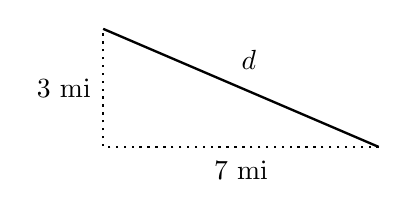
\begin{tikzpicture}
	\node at (-1.75,-0.3) {7~mi}; 
	\node at (-4.0,0.75) {3~mi};
	\node at (-1.65,1.1) {$d$};
	\draw[line width=0.03cm,dotted] (0,0) -- (-7/2,0) -- (-7/2,3/2);
	\draw[line width=0.03cm] (0,0) -- (-7/2,3/2);
	\end{tikzpicture}
	\]
We travel the solid line. Using the Pythagorean Theorem, the distance we will travel, $d$, is\dots
	\[
	d^2= a^2 + b^2= (3 \text{ mi})^2 + (7 \text{ mi})^2= 9 \text{ mi}^2 + 49 \text{ mi}^2= 58 \text{ mi}^2 \Longrightarrow d= \sqrt{58 \text{ mi}^2} \approx 7.61577 \text{ mi}
	\]
But we know that $d= vt$. Therefore, we have\dots \pspace
	\[
	\begin{gathered}
	d= vt \\[0.3cm]
	7.61577 \text{ mi}= 2.5 \text{ mph} \cdot t \\[0.3cm]
	t= \frac{7.61577 \text{ mi}}{2.5 \text{ mph}} \\[0.3cm]
	t= 3.046308 \text{ hrs}
	\end{gathered}
	\] \pspace
Therefore, it will take 3.046308~hours to walk to the lighthouse, i.e. 3~hours, 2~minutes, and 46.7~seconds to walk to the lighthouse. 



% Question 19 
\newpage
\question[5] Find the perimeter and area of the figure below. 
	\[
	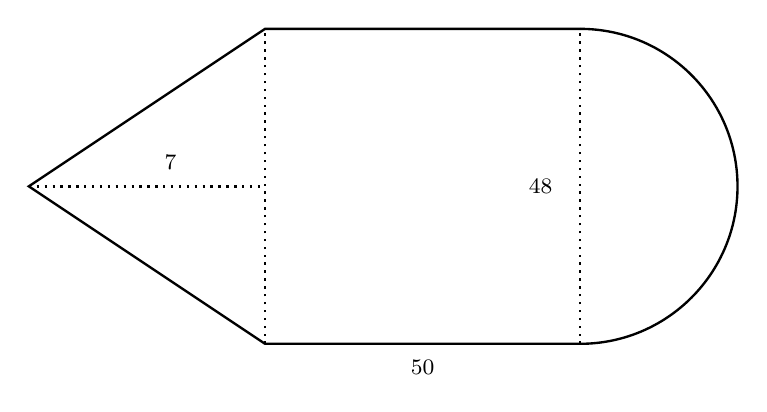
\begin{tikzpicture}
	\draw[line width=0.03cm] (4,-2) -- (0,-2) -- (-3,0) -- (0,2) -- (4,2);
	\draw[line width=0.03cm] (4,-2) arc(-90:90:2);
	
	\draw[line width=0.03cm,dotted] (-3,0) -- (0,0);
	\draw[line width=0.03cm,dotted] (0,-2) -- (0,2);
	\draw[line width=0.03cm,dotted] (4,-2) -- (4,2);
	
	\node at (-1.2,0.3) {\footnotesize 7};
	\node at (2,-2.3) {\footnotesize 50};
	\node at (3.5,0) {\footnotesize 48};
	\end{tikzpicture}
	\] \pspace

\sol We can use the symmetry of the diagram to fill it a bit more information:
	\[
	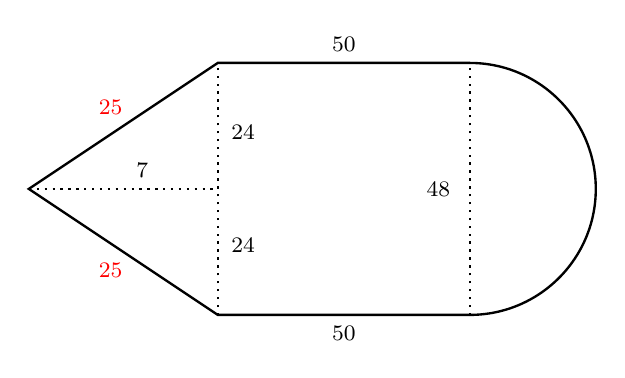
\begin{tikzpicture}[scale=0.8]
	\draw[line width=0.03cm] (4,-2) -- (0,-2) -- (-3,0) -- (0,2) -- (4,2);
	\draw[line width=0.03cm] (4,-2) arc(-90:90:2);
	
	\draw[line width=0.03cm,dotted] (-3,0) -- (0,0);
	\draw[line width=0.03cm,dotted] (0,-2) -- (0,2);
	\draw[line width=0.03cm,dotted] (4,-2) -- (4,2);
	
	\node at (-1.2,0.3) {\footnotesize 7};
	\node at (2,-2.3) {\footnotesize 50};
	\node at (3.5,0) {\footnotesize 48};
	\node at (0.4,0.9) {\footnotesize 24};
	\node at (0.4,-0.9) {\footnotesize 24};
	\node at (2,2.3) {\footnotesize 50};
	\node at (-1.7,1.3) {\footnotesize \color{red} 25};
	\node at (-1.7,-1.3) {\footnotesize \color{red} 25};
	\end{tikzpicture}
	\] 

We need to find the hypotenuse, $c$, of the triangle. We can use the Pythagorean Theorem:
	\[
	c^2= a^2 + b^2= 7^2 + 24^2= 49 + 576= 625 \Longrightarrow c= \sqrt{625}= 25
	\]
We know that a perimeter of a circle is $C= \pi d$. The perimeter of the half circle is then $\frac{1}{2}C= \frac{1}{2} (\pi d)= \frac{d}{2} \pi= r \pi$. But then the perimeter is\dots
	\[
	P= 50 + 25 + 25 + 50 + 24\pi= 150 + 24\pi \approx 225.398
	\]
The area of the region is\dots
	\[
	\begin{aligned}
	A&= A_{\Delta} + A_{\Box} + \frac{1}{2} A_{\bigcirc} \\[0.3cm]
	&= \frac{1}{2} bh + \ell w + \frac{1}{2} \cdot \pi r^2 \\[0.3cm]
	&= \frac{1}{2} \cdot 48 \cdot 7 + 50 \cdot 48 + \frac{1}{2} (24)^2 \pi \\[0.3cm]
	&= 168 + 2400 + 288\pi \\[0.3cm]
	&= 2568 + 288\pi \\[0.3cm]
	&\approx 3,\!472.78
	\end{aligned}
	\]



% Question 20
\newpage
\question[5] Compute the volume and surface area of the figure below. 
	\[
	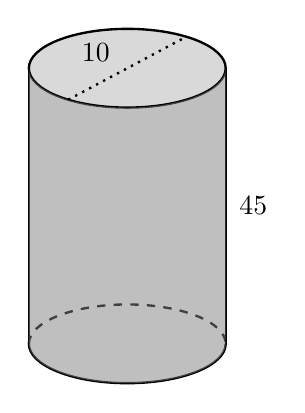
\begin{tikzpicture}
	\draw[line width= 0.03cm,fill=gray!30] (0,3.5) ellipse (1.25 and 0.5);	% Top
	\draw[line width= 0.03cm] (-1.25,3.5) -- (-1.25,0); % Left Side
	\draw[line width= 0.03cm] (1.25,0) -- (1.25,3.5);  % Right Side
	\draw[line width= 0.03cm] (-1.25,0) arc (180:360:1.25 and 0.5); % Bottom 
	\draw[line width= 0.03cm, dashed] (-1.25,0) arc (180:360:1.25 and -0.5); % Bottom Dotted
	\fill[gray,opacity=0.5] (-1.25,3.5) -- (-1.25,0) arc (180:360:1.25 and 0.5) -- (1.25,3.5) arc (0:180:1.25 and -0.5); % Gray Fill
	
	\draw[line width= 0.03cm,dotted] (-0.75,3.1) -- (0.75,3.9); % Top Dotted
	
	% Labels
	\node at (-0.4,3.7) {10};
	\node at (1.6,1.75) {45};
	\end{tikzpicture}
	\] \pspace

\sol Examining the cylinder above, we see that the cylinder has radius $\frac{10}{2}= 5$. We have\dots
	\[
	\begin{aligned}
	V&= \pi r^2 h \\[0.3cm] 
	V&= \pi (5^2) 45 \\[0.3cm]
	V&= \pi \cdot 25 \cdot 45 \\[0.3cm]
	V&= 1125 \pi \\[0.3cm]
	V&\approx 3534.29
	\end{aligned}
	\] \pspace
The surface area of a cylinder is\dots \pspace
	\[
	\begin{aligned}
	\text{S.A.}&= 2\pi r^2 + 2\pi r h \\[0.3cm]
	&= 2\pi (5^2) + 2 \pi (5) 45 \\[0.3cm]
	&= 50\pi + 450\pi \\[0.3cm]
	&= 500\pi \\[0.3cm]
	&\approx 1,\!570.8
	\end{aligned}
	\]


\end{questions}
\end{document}